\documentclass[11pt,a4paper,twoside]{article}
\usepackage[margin=1in, headheight=14pt]{geometry}
\usepackage{amsfonts,amsmath,amssymb,suetterl}
\usepackage{lmodern}
\usepackage[T1]{fontenc}
\usepackage{fancyhdr}
\usepackage{float}
\usepackage[utf8]{inputenc}
\usepackage{fontawesome}
\usepackage{enumerate}
\usepackage{xcolor}
\usepackage{hyperref}
\usepackage{tikz}
\usetikzlibrary{patterns, arrows.meta}

\DeclareUnicodeCharacter{2212}{-}

\usepackage{mathrsfs}
\usepackage[nodisplayskipstretch]{setspace}

\setstretch{1.5}
\renewcommand{\footrulewidth}{0pt}

\parindent 0ex
\setlength{\parskip}{1em}
\pagestyle{empty}

\begin{document}
    %
	\begin{singlespace}
		\begin{center}
			\Huge Queen Mary\\
			\LARGE University of London
		\end{center}
		\Large \textbf{MTH5123} \hfill \Large \textbf{Differential Equations,} \hfill \Large \textbf{Autumn 2020}\\
		\large \textbf{Coursework 3\_Week 5 part} \hfill \large \textbf{W. Huang}
		\rule{\textwidth}{0.4pt}
	\end{singlespace}
	%
	\begin{itemize}
		\item Each Coursework consists of three parts:
		\begin{enumerate}[\bfseries I.]
			\item Practice problems (you will get help on this part in Week 6 session 4. You should work on this before you go to this session.)
			\item Homework problems (to be submitted through QMquiz under QMplus > week 5)
			\item Exploration problems (to help you understand concepts discussed during lecture, not optional and examinable)
		\end{enumerate}
		\item \textcolor{red}{You must submit Week 5 and 6 homework problems of Coursework 3 together through the corresponding QMplus quiz under week 5 before the deadline, which is on the Friday afternoon of week 9 (Nov. 20th, 17:00). Otherwise, you will receive 0 for this coursework (which worths 5\% for your final mark). The correct answer will be shown in QMquiz after the submission deadline. Feedbacks about common mistakes will be discussed in the subsequent session 4 of week 10 after the reading week.}
		\item You have to solve the homework problems by yourself. \textit{Submitting homework questions on time is critical for you to achieve good grade in this module}
		\item A selection of solutions to coursework problems will be posted on QMPlus after the homework deadline. \textcolor{blue}{You are expected to seek solutions to the remaining problems using the Reading List and making use of our interactive session 4 in each week.}
		\item I encourage all students to learn and check your computational answers using math softwares such as MAPLE, Mathematica, MATLAB, etc. For example, there are free Mathematica licenses for students in QMUL. \href{https://www.its.qmul.ac.uk/services/service-catalogue/items/software---computational-mathematica.html}{\textcolor{blue}{Click here for the QMUL Mathematica software webpage.}} Using these softwares is a fun practice and will help you to visualise your solutions (– \textcolor{blue}{sketching solutions will be tested in the final exam}).
	\end{itemize}
	\rule{\textwidth}{0.4pt}
	%
	\textbf{I. Practice Problems}\par
	\textit{Question A is for learning content of week 3 - 4. Since many of you think Picard-Lindel\"{o}f Theorem is difficult, we add another question here. Since we already explained this in details in week 3 session 2 \& 4, week 4 session 2 \& 4, we will not discuss this question in our lectures, but you can discuss with your tutors in details again in your week 8 tutorials after the reading week.}
	\begin{enumerate}[\bfseries A.]
		\item Consider the initial value problem (IVP) $y^\prime = \frac{1}{2}y^{-1}\ (y\in \mathbb{R}),\ y(0) = 0$.
		%
	\begin{enumerate}[\bfseries 1)]
		\item Use the Picard-Lindel\"{o}f Theorem to justify existence and uniqueness of the solution to this ODE (without exhibiting the solution).
		\item Now solve the IVP. Find and sketch all possible solutions if the solution is not unique.
		\item Change the initial condition to$ y(0) = b$ where $b \neq 0$, graph the solution of this new IVP.
	\end{enumerate}
	%
	\item Assuming $x > 0$ write down the general solution to the Euler-type equations
	%
	\begin{enumerate}[\bfseries 1)]
		\item $x^2\frac{d^2y}{dx^2} - 4x\frac{dy}{dx} + 6y = 0$.
		\item $x^2y^{\prime\prime} - xy^\prime - 3y = 0$.
	\end{enumerate}
	%
	\item Find the general solutions of the second order inhomogeneous differential equations:
	%
	\begin{enumerate}
		\item $y^{\prime\prime} + 6y^\prime + 8y = -3e^{-x}$
		\item $y^{\prime\prime} + 7y^\prime + 6y = 10\sin(2x)$
	\end{enumerate}
	%
	\item Solve the following initial value problem:
	$$
	y^{\prime\prime} + 4y^\prime + 5y = 1 - 5x,\quad y(0) = 0,\ y^\prime(0) = -1
	$$
	\item Find the general solution of the second-order inhomogeneous differential equation using variation of paramter
	$$
	y^{\prime\prime} + 3y^\prime + 2y = e^{-2x}\cos x.
	$$
	\end{enumerate}
	\textbf{Note:}
	$$
	\int e^{ax}\cos \beta x dx = \frac{\beta}{\alpha^2+\beta^2}e^{\alpha x}\left(\sin \beta x + \frac{\alpha}{\beta}\cos \beta x\right),\quad \alpha \neq \pm i\beta
	$$
	whereas for $\alpha = \pm \beta$ it holds
	$$
	\int e^{\pm i\beta x} \cos \beta x dx = \frac{x}{2} + \frac{1}{4\beta}\sin 2\beta x \mp \frac{i}{4\beta} \cos 2\beta x.
	$$
	\textbf{II. Homework}\\
	Submit the third QM quiz under MTH5123 qmplus page > Week 5\\
	\rule{\textwidth}{0.4pt}
	%
	\textbf{III. Further Exploration: The application of ODEs on Newton’s Second Law}\\
	We consider a problem of great importance for applications: the motion of a mass attached to an elastic string under the influence of a periodic driving force, which we have discussed the equations in the lecture (week 1) about Newton’s Second Law. Here, we explore the solutions using the methods we learned in week 4 and 5.\par
	\textbf{Motion under periodic driving force and the resonance phenomenon}\par
	We consider differential equations for functions $y(t)$ of an independent variable time $t \in [0,\infty)$. Let us recall that for a point mass $m$ moving along a vertical coordinate $y$ under the influence of a force $f$ Newton’s Second Law is $\textbf{\text{mass}}\times \textbf{\text{acceleration}} = \textbf{\text{force}}$. This yields a second-order differential equation
	$$
	m\ddot{y} = f(t,y),
	$$
	where we will assume for simplicity that there is no friction in the system. Thus, the force $f$ depends on time and position but not on velocity $\dot{y}$. where we will assume for simplicity that there is no friction in the system. Thus, the force $f$ depends on time and position but not on velocity $\dot{y}$. To uniquely determine the motion of this system one has to specify initial conditions, which here are the initial value of the coordinate $y(t = 0)$ and the value of initial speed (velocity) $\dot{y}(t = 0) = v_0$. The
	% spring figure
	\begin{figure}[H]
		\centering
		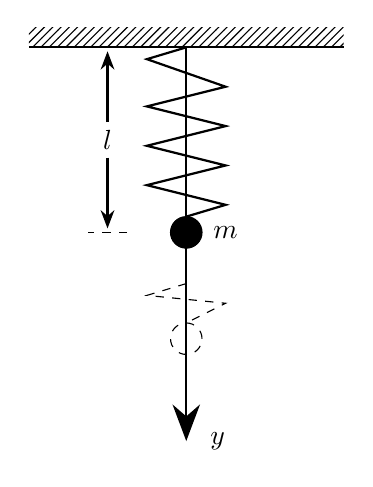
\begin{tikzpicture}
			\pattern[pattern=north east lines] (0,0) rectangle (4,.25);
			\draw[thick] (0,0) -- (4,0);
			\draw[thick,-{Stealth[scale=2]}] (2,0) -- (2,-5);
			\draw[thick] (2,0) -- (1.5,-.15) -- (2.5,-.5) -- (1.5,-.75)--(2.5,-1)--(1.5,-1.25)--(2.5, -1.5)--(1.5,-1.75)--(2.5, -2)--(2,-2.15);
			\draw[fill] (2,-2.35) circle [radius =0.2];

			\draw[dashed] (2,-3)--(1.5, -3.15)--(2.5,-3.25)--(2, -3.5);
			\draw[dashed] (2,-3.7) circle [radius =0.2];

			\draw[dashed] (1.25,-2.35) -- (0.75,-2.35);

			\node at (1,-1.175) {$l$};
			\draw[thick,-{Stealth[scale=1]}] (1,-1.4) -- (1,-2.3);
			\draw[thick,-{Stealth[scale=1]}] (1,-.95) -- (1,-.05);

			\node at (2.5,-2.35) {$m$};
			\node at (2.4,-5) {$y$};
		\end{tikzpicture}
		%
		\caption{Sketch of a spring-mass system.}\label{1}
	\end{figure}
	simplest system of this type is represented by a point mass $m$ attached to the loose end of an elastic spring of length $l$, with the other end of the spring fixed to a ceiling; see Fig. \ref{1}. To keep our considerations as simple as possible we also neglect any additional external driving force acting on the mass. Measuring the coordinate $y$ from the ceiling downwards, the mass is then subject to a force equal to the sum of only two contributions: the position-independent \textbf{gravity force} $f_g = mg$ and the position dependent \textbf{elastic force} $f_{el} = -k(y-l)$ (Hooke’s law of elasticity).\par
	\textbf{Question:} Using the constant parameters $k,\ m,\ g,\ l$, write down the second ODE linear ODE of the position of the point mass $y$ over time $t$ for the above system. Find the general solution to this ODE, and the solution to the IVP with the initial position and speed at $t = 0$ as $y(0) = y_0,\ \dot{y}(0) = 0$. Here, $y_0$ is a given constant number.\\
	(Hint: you first need to identify the variable and independent variable. The ODE can be solved by second order linear ODE methods.)


\end{document}